

%\chapter{Domain shift in CT images}
\chapter{Mitigating Domain Shift from CT Reconstruction Kernels}
\label{chap:ct}

%Domain shift is one of the most salient challenges in medical computer vision. Due to immense variability in scanners’ parameters and imaging protocols, even images obtained from the same person and the same scanner could differ significantly.
In this chapter, we consider variability in computed tomography (CT) images caused by different convolution kernels used in the reconstruction process, the critical domain shift factor in CT. The choice of convolution kernel affects pixel granularity, image smoothness, and noise levels, resulting in images that, while anatomically identical, differ in style.

We analyze several datasets of paired CT images where smooth and sharp images were reconstructed from the same sinograms using different kernels. Despite identical anatomy, the consistency between predictions on these paired images is surprisingly low, with an average Dice score of just $0.46$. Furthermore, we observe a significant decline in COVID-19 segmentation accuracy when models are trained and tested on different reconstruction kernels.

To address this domain shift, we propose two methods. The first is Filtered Back-Projection Augmentation (FBPAug), a novel knowledge-driven augmentation technique designed to simulate domain shifts associated with varying reconstruction kernels. \text{FBPAug} improves prediction consistency from a Dice score of $0.46$ to $0.76$, surpassing other augmentation methods. The second method, F-Consistency, is an unsupervised domain adaptation (DA) approach that leverages paired, unlabeled CT images reconstructed with different kernels. This method enforces similarity in the network’s hidden representations by minimizing the mean squared error (MSE) between feature maps of paired images. Given sufficient paired data, F-Consistency further enhances prediction consistency to a Dice score of $0.80$, outperforming FBPAug, other unsupervised DA methods, and demonstrating superior generalization to unseen kernels.

The results presented in this chapter are based on the author’s publications~\cite{saparov2021zero,shimovolos2022adaptation}.


\section{Background}

Computed tomography (CT) is a widely used method for medical imaging. CT images are reconstructed from the raw acquisition data, represented in the form of a sinogram. Sinograms are two-dimensional profiles of tissue attenuation as a function of the scanner's gantry angle. Here, one of the most common reconstruction algorithms is Filtered Back Projection (FBP) \cite{schofield2020image}. This algorithm has an important free parameter called \textit{convolution kernel}. The choice of a convolution kernel defines a trade-off between image smoothness and noise level \cite{schaller2003spatial}. Reconstruction with a high-resolution kernel yields \textit{sharp} pixels and a high noise level. In contrast, usage of a lower-resolution kernel results in \textit{smooth} pixels and a low noise level. Depending on the clinical purpose, radiologists use different kernels for image reconstruction.

Modern deep neural networks (DNN) are successfully used to automate computing clinically relevant anatomical characteristics and assist with disease diagnosis. However, DNNs are sensitive to changes in data distribution which are known as \textit{domain shift}. Domain shift typically harms models' performance even for simple medical images such as chest X-rays \cite{zech2018variable}. In CT images, factors contributing to domain shift include slice thickness and inter-slice interval, different radiation dose, and reconstruction algorithms, e.g., FBP parameters \cite{kloenne2020domain}. The latter problem is a subject of our interest.
%One could perceptually compare the same image reconstructed with two different kernels in Figure~\ref{fig:consistency_preds}, e.g., B1 and B2.

Recently, several studies have reported a drop in the performance of convolutional neural networks (CNN), trained on \textit{sharp} images while being tested on \textit{smooth} images, e.g., in lung cancer \cite{choe2019deep} and emphysema segmentation \cite{lee2019ct}. The authors of \cite{sandfort2019data} proposed using generative adversarial networks (GAN) to generate realistic CT images imitating arbitrary convolution kernels. A more straightforward approach, simultaneously proposed in \cite{missert2019simulation}, \cite{choe2019deep}, and \cite{lee2019ct}, suggests using a CNN to convert images reconstructed with one kernel to images reconstructed with another. Later, such image-to-image networks can be used either as an augmentation during training or as a preprocessing step during inference.

In this chapter, we show that the domain shift induced by the difference in reconstruction kernels also decreases the quality of the COVID-19 segmentation algorithms. To do so, we construct two domains from the publicly available data: the \textit{source} domain with the \textit{smooth} reconstruction kernels and \textit{target} domain with the \textit{sharp} reconstruction kernels. We train the segmentation model on the source domain and test it on the target domain and validate the most relevant DA methods. In our comparison, we include all related augmentation methods, unsupervised adversarial learning \cite{ganin2015unsupervised}, and two proposed methods \cite{saparov2021zero,shimovolos2022adaptation}.
 
The first proposed method is FBP Augmentation (FBPAug), a novel augmentation method based on the FBP reconstruction algorithm. This augmentation mimics processing steps used in proprietary manufacturer's reconstruction software. We initially apply Radon transformation to all training CT images to obtain their sinograms. Then, we reconstruct images using FBP but with different randomly selected convolution kernels. To show the effectiveness of our method, we compare segmentation masks obtained on a set of paired images, reconstructed from the same sinograms with different convolutional kernels.%These paired images are perfectly aligned; the only difference is their style, smooth or sharp.

We note that the large pools of unlabeled chest CT image pairs which differ only in reconstruction kernels within every pair are publicly available, e.g., \cite{morozov2021simplified}. The intuition here is that the adaptation methods should outperform the augmentation one when a broader range of real-world data is available. Specifically, in such conditions, we propose the second method which enforces the cross-domain feature maps consistency between paired images; we call our method F-Consistency. F-Consistency minimizes the mean squared error (MSE) between the network’s hidden representations (feature maps) of paired images. We expect that explicitly enforcing consistency on the paired images should outperform the adversarial learning that emulates similar behavior minimizing the adversarial loss.

%Our work highlights a domain shift problem in the COVID-19 segmentation task and suggests an efficient solution to this problem. These are our three main contributions:
%% We summarize our three main contributions as follows:
%
%\begin{itemize}
%	
%	\item Firstly, we demonstrate that the difference in CT reconstruction kernels affects the segmentation quality of COVID-19 lesions. The model without adaptation achieves only a $0.56$ Dice Score on the unseen domain, while the best adaptation methods scores $0.64$. In terms of similarity between predictions on the paired images, the baseline Dice Score is $0.46$, which is almost two times lower than the $0.80$ achieved by our method.
%	
%	\item Secondly, we propose FPBAug, a knowledge-driven and efficient approach to augment CT images in sinogram space, emulating reconstruction with different kernels. We show that our method outperforms other augmentation approaches. Moreover, neither specific preparation of source domain data nor target domain data is required, so our publicly released \href{https://github.com/STNLd2/FBPAug}{FBPAug} can be used as a plug-and-play module for zero-shot domain adaptation in CT-based tasks.
%	
%	\item Thirdly, we propose the flexible adaptation approach that outperforms the other considered methods when provided with enough unlabeled data. We also show that our method better generalizes to unseen CT reconstruction kernels and it is less sensitive to the absence of the semantic content (COVID-19 lesions) than the other methods trained on unlabeled data.
%	
%\end{itemize}


\section{Methods}

\subsection{Filtered Back-Projection Augmentation}


We begin by recalling the discrete formulation of the inverse Radon transform, known as the Filtered Back-Projection (FBP) algorithm. In analytical Computed Tomography (CT), FBP provides an explicit inversion of the projection operator under the assumption of parallel-beam geometry. The algorithm consists of two consecutive operations: (i) filtering of the measured projection data, and (ii) reconstruction of the attenuation map by the Back-Projection (BP) operator. In the continuous setting, both operations correspond to well-defined integral transforms, whereas in practice they are implemented in discrete form for a finite set of projection angles.

In the ideal continuous case, reconstruction requires filtering the projection data prior to back-projection in order to compensate for the frequency attenuation inherent in the Radon transform. The optimal filter in the noise-free setting is the so-called \textit{ramp filter}, whose frequency response grows linearly with spatial frequency, thereby restoring high-frequency components corresponding to sharp tissue boundaries. Denoting the ramp kernel by $\kappa(t)$, its Fourier transform is given by

\[
\mathcal{F}[\kappa(t)](w) = |w|.
\]

This ideal filter amplifies high-frequency components and is thus highly sensitive to noise, motivating the use of smoothed or modified filters in practical CT systems.

Under these assumptions, the reconstructed attenuation map, i.e., image, $I(x, y)$ is obtained as

\begin{equation}
	\label{eq:main_eq}
	I(x, y) = \text{FBP}(p_\theta(t)) = \text{BP}(p_\theta(t) * \kappa(t)),
\end{equation}

\noindent
where $t = t(x,y) = x\cos\theta + y\sin\theta$ and $*$ denotes convolution along the detector coordinate. This expression follows directly from the Fourier Slice Theorem, which relates the 1D Fourier transform of a projection to a central slice of the 2D Fourier transform of the original image. And $p_{\theta} (t) = \mathcal{R}[I](t, \theta)$ denote the projection (Radon transform) of the image at angle $\theta$.

In the discrete case, let a finite set of projection angles be given by $\theta_i = (i - 1) \Delta \theta$, with uniform spacing $\Delta \theta = \pi / n$. The discrete Back-Projection operator acts on a family of filtered projections $\{ p_{\theta_i} (t)\}_{i=1}^n$, as

\[
BP(p_\theta(t))(x, y) = \frac{\Delta\theta}{2\pi}\sum\limits_{i=1}^n p_{\theta_i}(x\cos\theta_i + y\sin\theta_i) \approx \frac{1}{2n}\sum\limits_{i=1}^n p_{\theta_i}(x\cos\theta_i + y\sin\theta_i),
\]

\noindent
where the normalization ensures that the discrete operator approximates the continuous integral over $[0, \pi)$.

It is important to note that the ramp kernel $\kappa(t)$ in \eqref{eq:main_eq} is a generalized function and cannot be expressed as an ordinary function because the integral of $|w|$ in inverse Fourier transform does not converge. Nevertheless, practical implementation relies on the convolution theorem, $\mathcal{F}(f*g) = \mathcal{F}(f)\cdot\mathcal{F}(g)$, and on the linearity of both the Fourier and Back-Projection (finite weighted sum) operators, which allows one to write

\[
\mathcal{F}^{-1}\mathcal{F}[I(x, y)] = \mathcal{F}^{-1}\mathcal{F}[\text{BP}(p_\theta * \kappa)] = \text{BP}(\mathcal{F}^{-1}\mathcal{F}[p_\theta * \kappa]) = \text{BP}(\mathcal{F}^{-1}\{\mathcal{F}[p_\theta]\cdot|w|\}),\]
\[I(x, y) = \text{BP}\left(\mathcal{F}^{-1}\{\mathcal{F}[p_\theta]\cdot|w|\}\right).\]

In real CT systems, the ideal ramp filter is replaced by a family of empirical filters that modulate the frequency response to suppress noise or enhance edges, commonly referred to as reconstruction kernels (e.g., ``soft'', ``standard'', or ``bone'' kernels). However, the exact analytical form of these kernels remains proprietary, as it constitutes part of the intellectual property of CT manufacturers.

But now, as the application of convolution filters in the frequency domain is mathematically defined, we can construct our own parametric family of kernels that approximate this behavior. This family allows for continuous control over the degree of sharpness or smoothness in the reconstructed image and provides an interpretable and reproducible alternative to vendor-specific filters.

We propose a family of convolution kernels $k_{a,b}$ with the following Fourier transform:

\[\mathcal{F}[k_{a,b}](w) = \mathcal{F}[\kappa](w)(1 + a \mathcal{F}[\kappa](w)^b) = |w|(1 + a|w|^b),\]

\noindent
where $a \in \R$ controls the degree of enhancement and $b > 0$ determines the spectral roll-off. For $a > 0$ and larger $b$, high frequencies are amplified, producing sharper images; for $a < 0$, the response is damped, yielding smoother reconstructions.

Finally, given a CT image $I$ reconstructed with an unknown or fixed kernel, we simulate its appearance under another kernel by applying the inverse Radon-transform-based operator

\[\hat{I}(x, y) = \text{BP}\left(\mathcal{F}^{-1}\{\mathcal{F}[\mathcal{R}(I)]\cdot\mathcal{F}[k_{a,b}]\}\right),\]

\noindent
where $\mathcal{R}(I)$ denotes the Radon transform of the image. Unlike purely spatial convolution augmentations, this formulation operates in the projection domain and therefore preserves the physical consistency of the CT acquisition model. Figure~\ref{fig:crops} illustrates the effect of applying sharpening augmentation to a soft-kernel image (Figure~\ref{fig:crops}(a) to (c)) and vice versa (Figure~\ref{fig:crops}(b) to (d)). The resulting images remain physically plausible while exhibiting controlled variations in contrast and edge sharpness, which enhances the robustness of downstream learning models to variations in reconstruction protocol.

%Here, $a$ and $b$ are the parameters that influence the sharpness or smoothness of an output image and $\mathcal{R}(I)$ is a Radon transform of image $I$. The output of the Radon transform is a set of projections. Fig. \ref{fig:crops} shows an example of applying sharping augmentation on a soft kernel image (Fig. \ref{fig:crops}(a) to (c)) and vice versa: applying softening augmentation on a sharp kernel image (Fig. \ref{fig:crops}(b) to (d)). 


\begin{figure}[h]
	\centering
	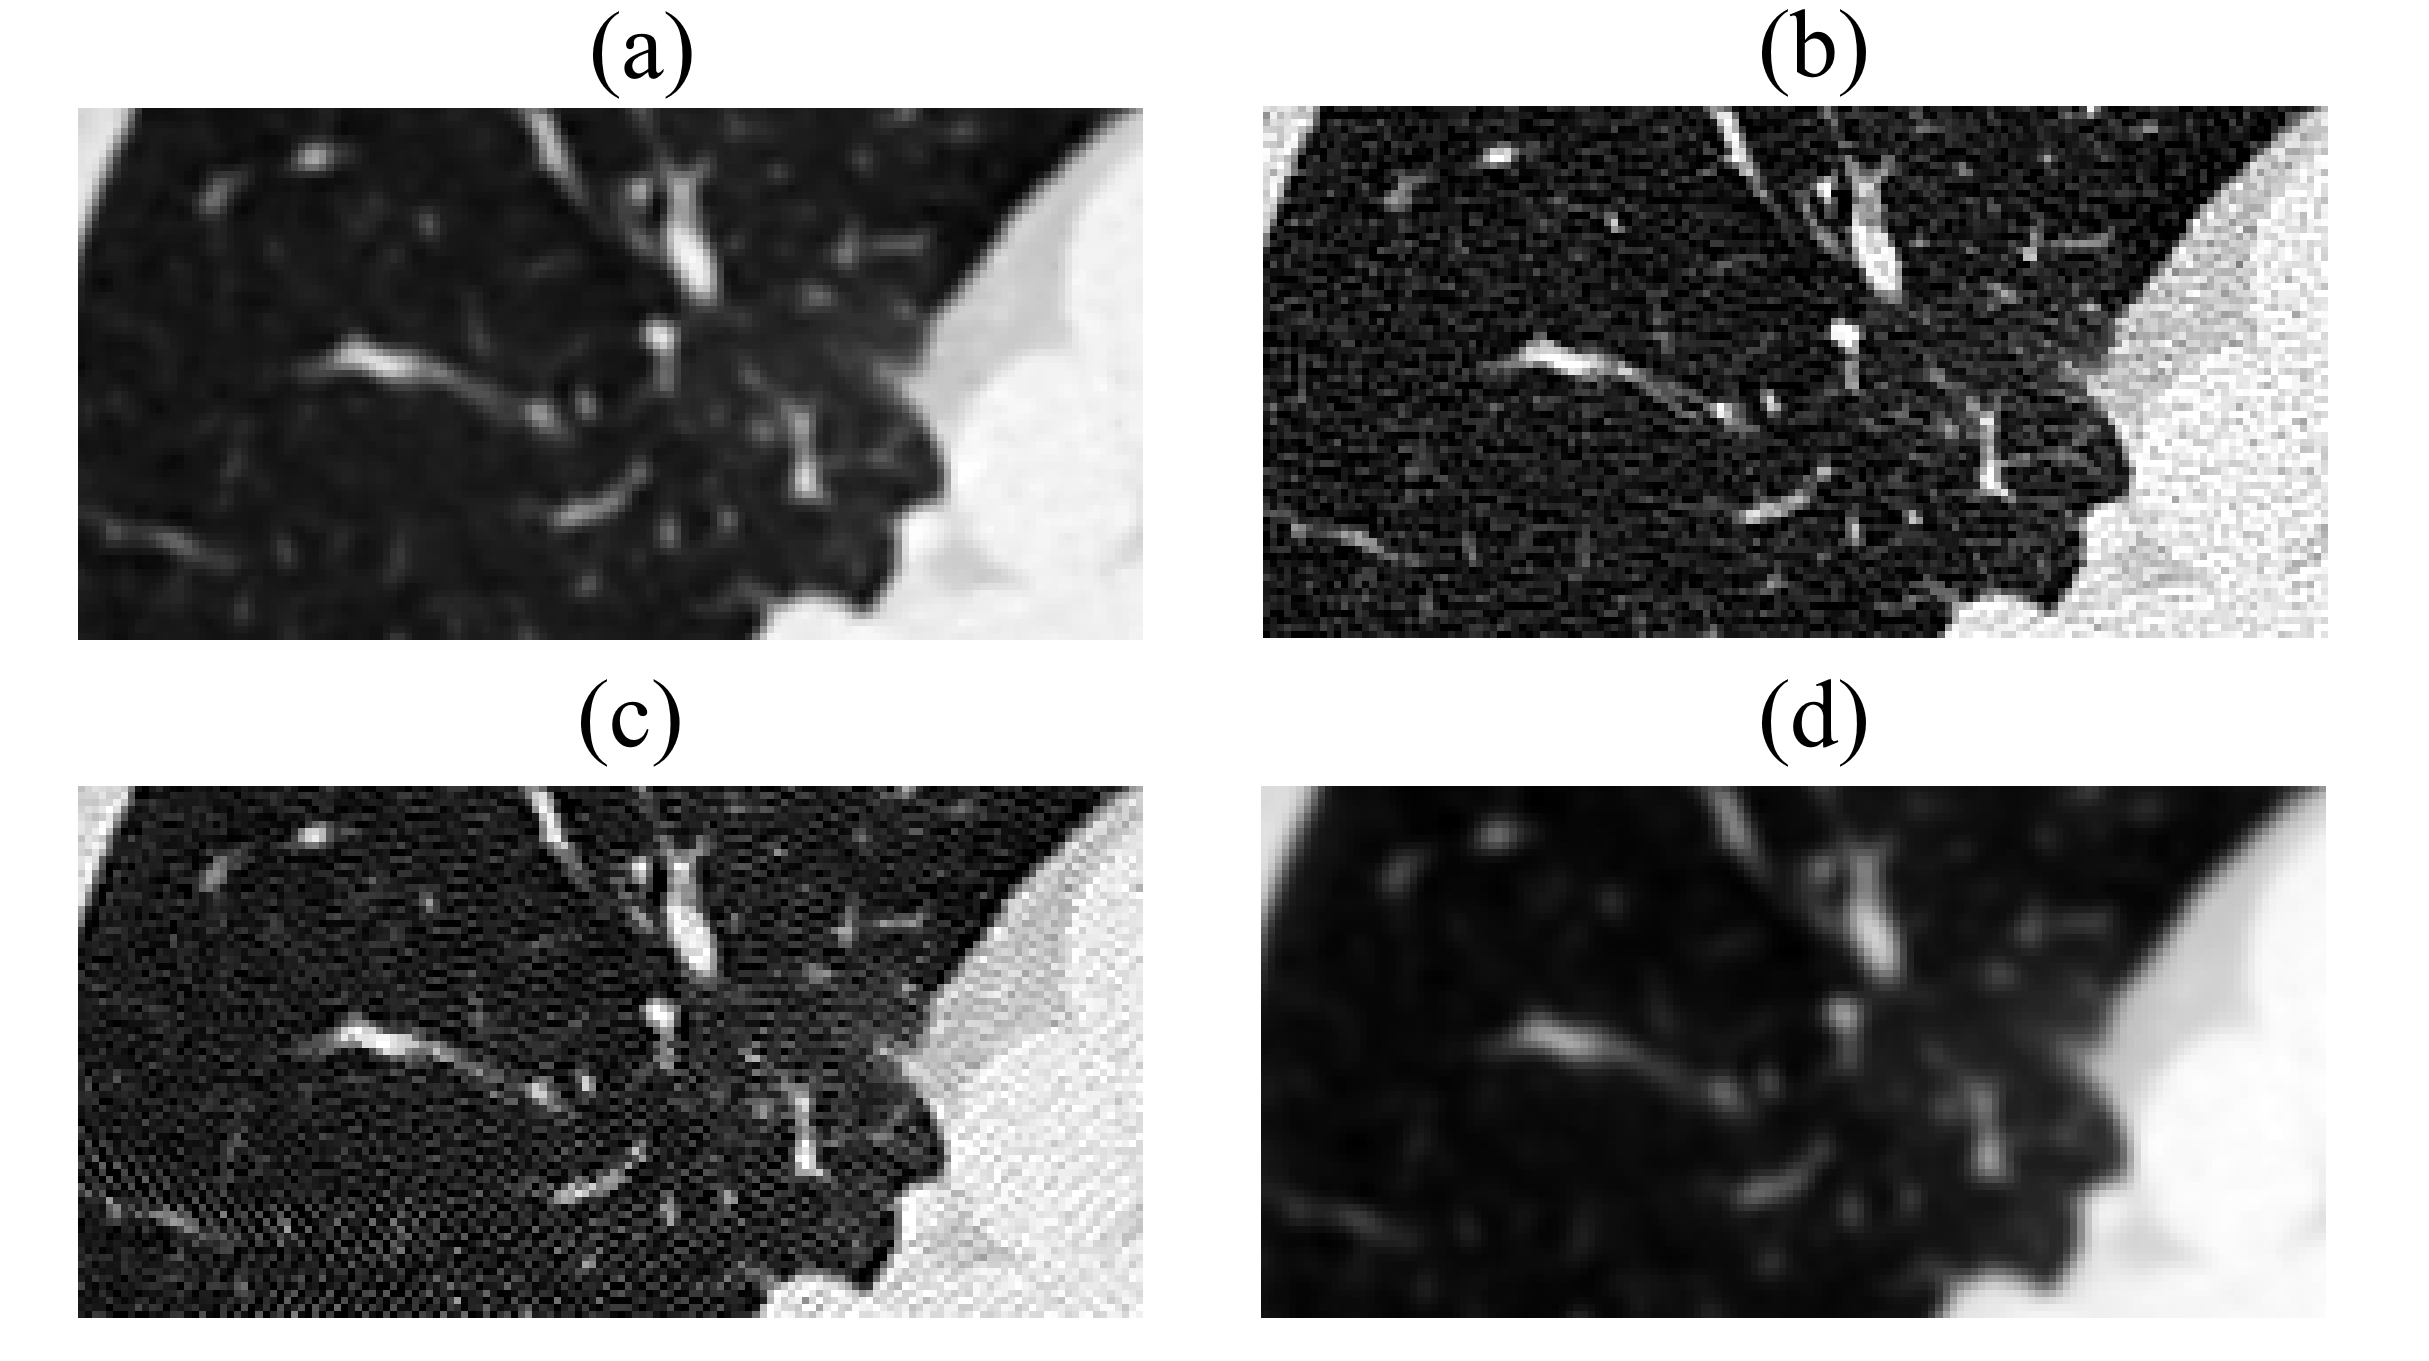
\includegraphics[width=\linewidth]{Dissertation/Figures/3_ct/4crops.png}%[width=7cm][width=7cm]
	\caption{\textbf{An example of paired CT slices (top row) and the effect of the augmentation by the proposed method (bottom row).} The top row contains original images: a slice reconstructed either with a smooth kernel (a) or sharp kernel (b). The bottom row shows augmented images: the top-left image processed by FBPAug with parameters $a=30,~b=3$ shifting it from smooth to sharp (c); the top-right image processed by FBPAug with parameters $a=-1,~b=0.7$ from sharp to smooth (d).}
	\label{fig:crops}
	\vspace{2\baselineskip}
\end{figure}



\subsection{Cross-Domain Features Consistency}

We train all segmentation methods using the annotated dataset $S_s = \{ ( x_i, y_i ) \}_{i=1}^{N_s}$, where $x$ is a volumetric CT image, $y$ is a corresponding binary mask, and $N_s$ is the total size of training dataset. The dataset $S_s$ consists of images reconstructed with smooth kernels; we call it source dataset. We test all methods using the annotated dataset $S_t = \{ ( x_i, y_i ) \}_{i=1}^{N_t}$. The dataset $S_t$ consists of the $N_t$ images reconstructed with the sharp kernels; we call it target dataset. Although $S_t$ contains annotations, we use them only to calculate the final score.

Adaptation methods use additional paired dataset $S_2 = \{ ( x_i, \tilde{x}_i ) \}_{i=1}^{N_2}$, which has no annotations. However, every image $x \in S_2$ has a paired image $\tilde{x}$ reconstructed from the same sinogram but with a different kernel. Here, we assume that $x$ belongs to the source domain and $\tilde{x}$ belongs to the target domain.

Similar to the adversarial approaches (e.g., \cite{ganin2015unsupervised}), we propose to remove style-specific kernel information from the feature maps. However, we additionally exploit the paired nature of the unlabeled dataset $S_2$. Instead of the adversarial loss, we minimize the distance between feature maps of paired images. Let us denote feature extractor $H_f$, the part of segmentation model that maps input images $x$ into the feature space, and segmentation head $H_p$, the complement part of segmentation model that predicts binary mask $\hat{y} = H_p \left( H_f \left( x \right) \right)$. Further, we denote the feature vector for every image $x$ as $f$, $f = H_f (x; \: \theta_f)$. For the paired image $\tilde{x}$, we use the similar notation $\tilde{f}$.%In Figure~\ref{fig:method_schematic}, $H_f$ and $H_p$ correspond to the encoder and decoder parts of the model, respectively.

During the training, we minimize the sum of segmentation loss and distance between paired features ($f$ and $\tilde{f}$). Thus, the optimization problem is
\begin{align}
	\label{eq:f-consistency_opt}
	\begin{split}
		E (\theta_f, \theta_p) &= \sum_{i = 1}^{N_s} L_s (H_p(H_f (x_i; \: \theta_f); \: \theta_p), \: y_i) \: \\
		& + \: \alpha \sum_{j = 1}^{N_2} L_c (H_f (x_j; \theta_{f}), \: H_f (\tilde{x}_j; \theta_f)) \\
		& = \sum_{i = 1}^{N_s} L_s \left(\hat{y}_i ,\: y_i \right) \: + \: \alpha \sum_{j = 1}^{N_2} L_c (f_j,\: \tilde{f}_j ),  
	\end{split} \\
	(\hat{\theta}_f, \hat{\theta}_p) & = \argmin_{\theta_f, \theta_p} E(\theta_f, \theta_p),
\end{align}
where $L_s$ is the segmentation loss (Binary Cross-Entropy) and $L_c$ is the consistency loss. For the consistency loss, we use mean squared error (MSE) between paired feature maps. Parameter $\alpha$ regulates the trade-off between two objectives. We call this method \textit{F-Consistency} since it enforces the consistency between paired feature maps.

We present our method schematically in Figure~\ref{fig:method_schematic}(5) along with the competitive approaches, e.g., Domain Adversarial Neural Network (DANN) \cite{ganin2015unsupervised}. Note that we do not need any additional model as discriminator in DANN in the case of F-Consistency. The features are aggregated from the same encoder layers as in DANN.

\begin{landscape}
\begin{figure}[p]
	\centering
	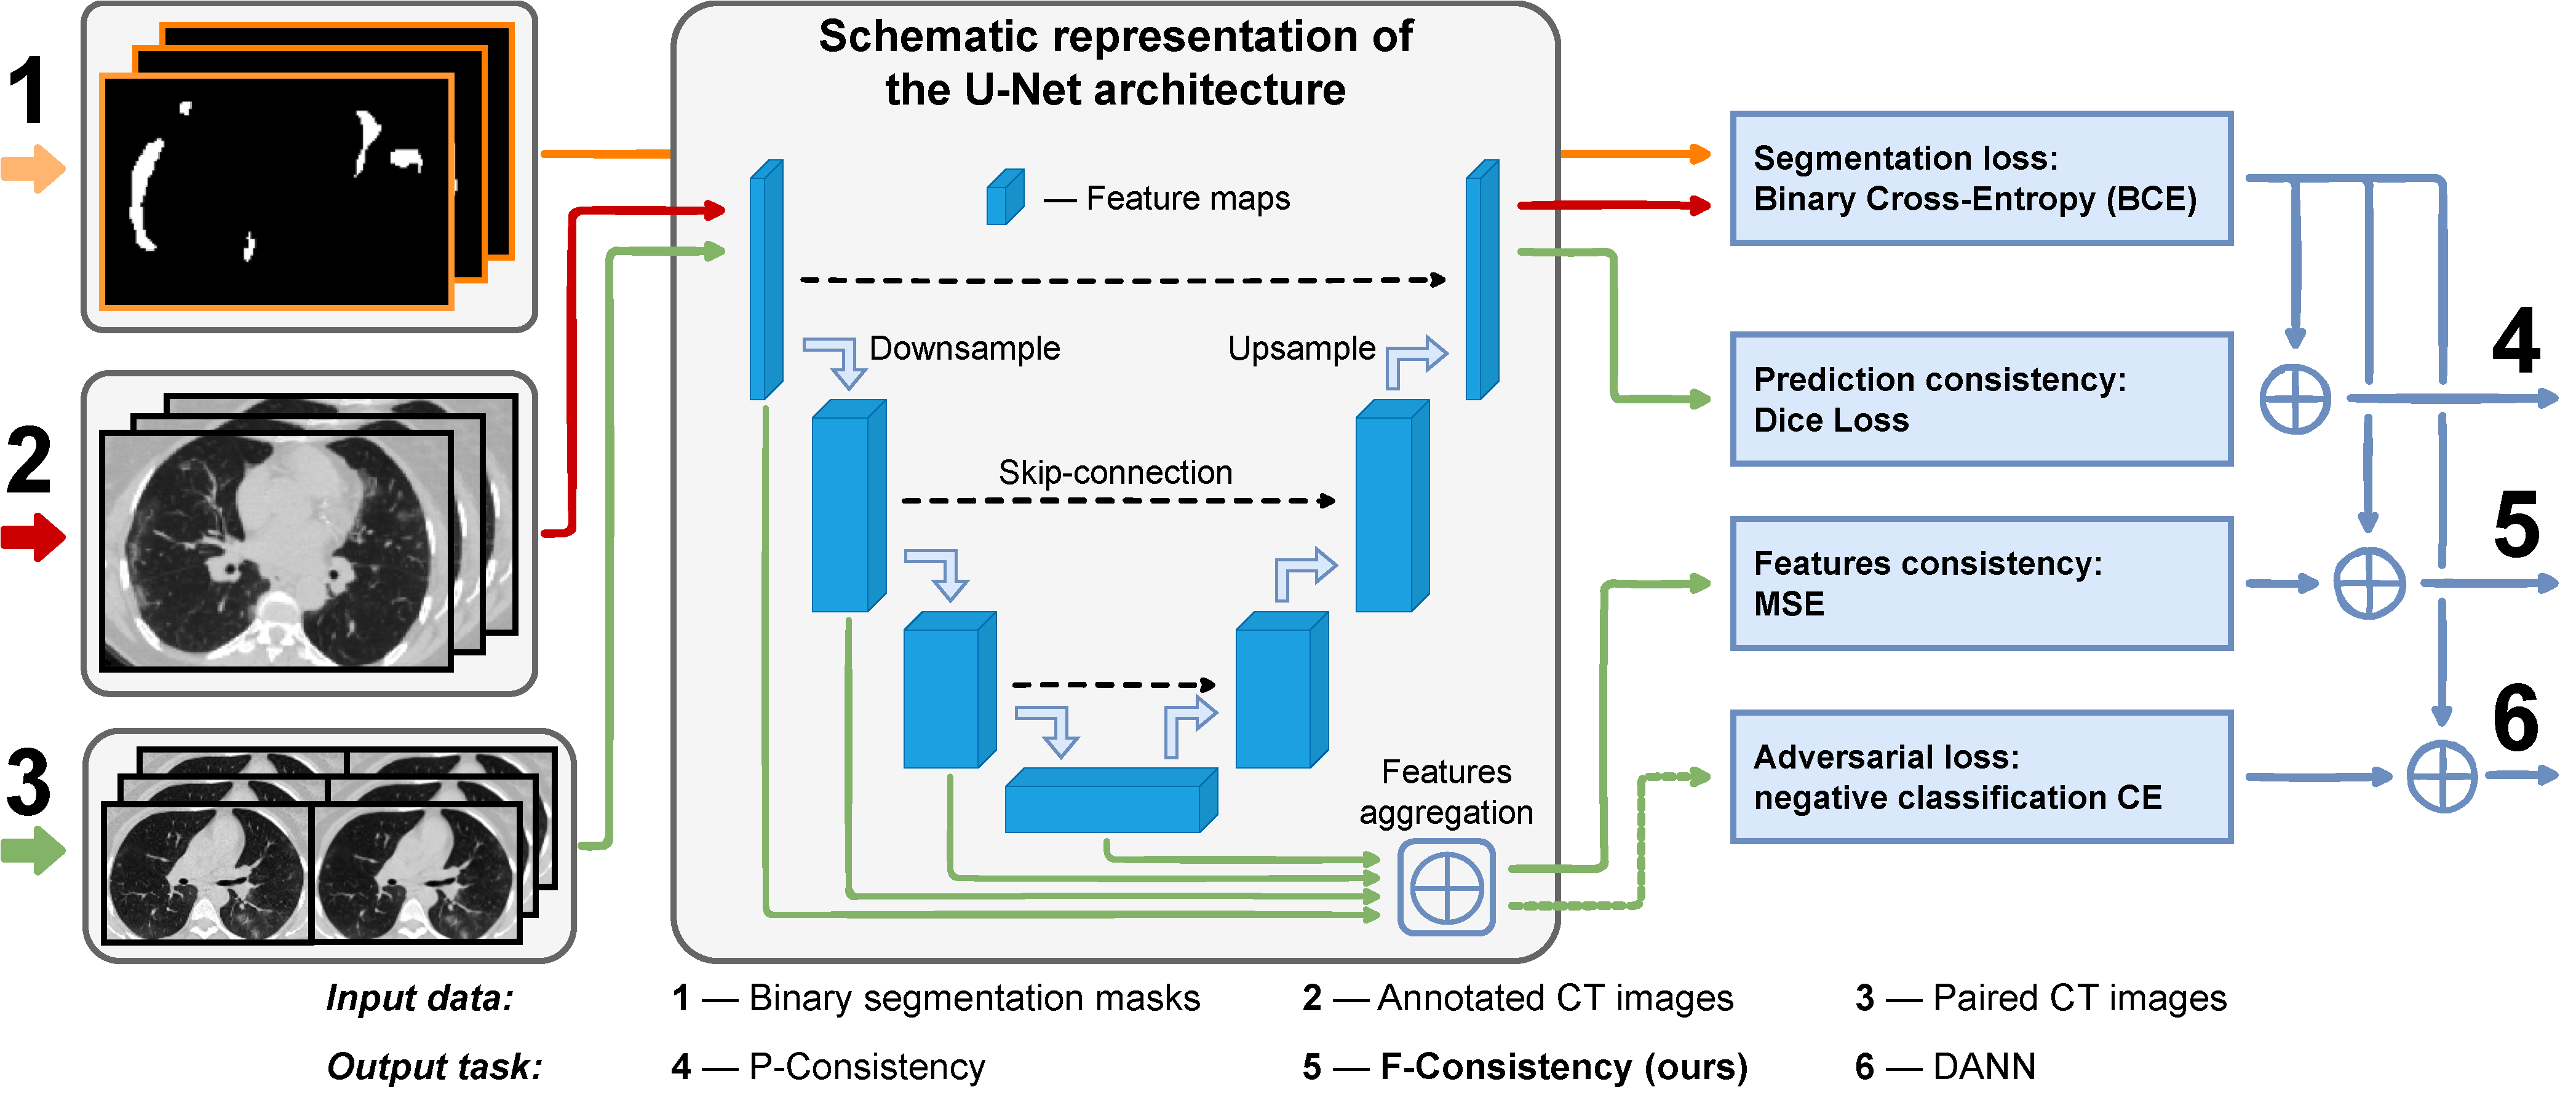
\includegraphics[width=\linewidth]{Dissertation/Figures/3_ct/method_schematic_4.pdf}
	\caption{Schematic representation of the proposed method, \textit{\textbf{F-Consistency}} (\textbf{5}), and its competitors, \textit{P-Consistency} (\textbf{4}) and \textit{DANN} (\textbf{6}). All methods build upon the same U-Net architecture, which we train to segment the COVID-19 binary mask (\textbf{1}) from the axial slices of chest CT images (\textbf{2}). These adaptation methods use unlabeled paired data (\textbf{3}) to improve the model performance on the target domain. We show the flow and different usage of the paired data in different methods with green.\label{fig:method_schematic}}
	%In the image, \textit{DANN} and \textit{F-Consistency} operate with the encoder layers but can be easily extended to the %decoder versions.
\end{figure}
\end{landscape}

\subsection{Cross-Domain Predictions Consistency}

A special case of F-Consistency is enforcing the consistency of paired predictions as the predictions are de facto the feature maps of the last network layer. This approach is proposed in \cite{orbes2019multi} also in the context of medical image segmentation. Further, we denote this method \textit{P-Consistency}. Visually, it could be compared with DANN and F-Consistency in Figure~\ref{fig:method_schematic}(4). The optimization problem is the same as in Equation~(\ref{eq:f-consistency_opt}), except $L_c$ is Dice Loss \cite{milletari2016v} and $f$ and $\tilde{f}$ are the last layer features, i.e., predictions.



\section{Data}

In our experiments, we use a combination of different datasets with chest CT images. The data could be divided into two subsets according to the experimental purposes. The first collection of datasets consists of images with annotated COVID-19 lesions, i.e., with binary masks of ground-glass opacity and consolidation. It serves to train the COVID-19 segmentation algorithms. The second collection consists of chest CT images which are reconstructed with different kernels but have no COVID-19 annotations. We filter the data into pairs of images reconstructed with the smooth and sharp kernels. This data is further used to adapt the models in an unsupervised manner.
% We detail every dataset of the segmentation collection in Section~\ref{ssec:data:segm}. 
% We detail the second collection in Section~\ref{ssec:data:paired}.


\subsection{Segmentation Data}

We use three publicly available datasets to train and test the segmentation algorithms: Mosmed-1110 \cite{morozov2020mosmeddata}, MIDRC \cite{tsai2021rsna}, and Medseg-9. We ensure that selected datasets contain original 3D chest CT imaging studies without third-party preprocessing artifacts. The images from the Mosmed-1110 and MIDRC datasets are reconstructed using smooth kernels, whereas Medseg-9 images have sharp reconstruction kernels. That allows us firstly to identify and then address the domain shift. We split the segmentation data into the source (COVID-train) and target (COVID-test) domains and describe them below. A summary of the segmentation datasets is presented in Table~\ref{tab:data_segm}.



%\begin{table}[H]
%	\centering
%	\caption{Summary of the segmentation datasets. {\textit{Effective size} means the number of annotated images after appropriate filtering.} \label{tab:data_segm}}
%	\newcolumntype{C}{>{\centering\arraybackslash}X}
%	\resizebox{\textwidth}{!}{%
%	\begin{tabularx}{\textwidth}{CCCCCC}
%		\toprule
%		\multirow{1.5}{*}{\textbf{Dataset}} & \multirow{1.5}{*}{\textbf{Source }}& \makecell{\textbf{Effective} \\ \textbf{Size}} & \multirow{1.5}{*}{\textbf{Kernels}} & \multirow{1.5}{*}{\textbf{Annotations}} &\multirow{1.5}{*}{ \textbf{Split}} \\
%		\midrule
%		\multirow{4}{*}{COVID-train} & \makecell{Mosmed-1110 \\ \cite{morozov2020mosmeddata}} & 50 & \makecell{unknown \\ smooth} & COVID-19 mask & \multirow{4}{*}{\makecell{5-fold \\ cross-val}} \\
%		\cmidrule(lr){2-5}
%		& \makecell{MIDRC \\ \cite{tsai2021rsna}} & 112 & \makecell{B/L/BONE/ \\ STANDARD \\ (smooth)} & COVID-19 mask & \\
%		\midrule
%		COVID-test & Medseg-9 & 9 & \makecell{unknown \\ sharp} & \makecell{COVID-19 mask, \\ lungs mask} & \makecell{hold-out \\ test} \\
%		\bottomrule
%	\end{tabularx}}
%\end{table}


\begin{table}[h]
	\centering
	\caption{Summary of the segmentation datasets.\label{tab:data_segm}}
	
	%\resizebox{\textwidth}{!}{%
		\begin{tabular}{c c c c c c}
			\toprule
			Dataset & Source & Size & Kernels & Annotations & Split \\
			\midrule
			\multirow{2}{*}[-1.0em]{\textit{COVID-train}} & Mosmed-1110 & 50 & \makecell{unknown \\ smooth} & COVID-19 & \multirow{2}{*}[-1.5em]{\makecell{5-fold \\ cross-val}} \\
			\cmidrule(lr){2-5}
			& MIDRC & 112 & \makecell{B/L/BONE/ \\ STANDARD \\ (smooth)} & COVID-19 & \\
			\midrule
			\textit{COVID-test} & Medseg-9 & 9 & \makecell{unknown \\ sharp} & \makecell{COVID-19, \\ lungs} & \makecell{hold-out \\ test} \\
			\bottomrule
			
	\end{tabular}%}
\end{table}


\textbf{Mosmed-1110.} This dataset consists of $1110$ chest CT scans collected in Moscow clinics during the first months of $2020$ \cite{morozov2020mosmeddata}. Scanning was performed on \textit{Canon (Toshiba) Aquilion 64} units using the standard scanner's protocol: inter-slice distance of $0.8$ mm and smooth reconstruction kernels in particular. However, the public version of Mosmed-1110 contains every $10th$ slice of the original series, which makes the resulting slice distance equal to $8.0$ mm. Additionally, the $50$ series have annotated binary masks depicting COVID-19 lesions (ground-glass opacity and consolidation). We use only these $50$ images in our experiments.
% Also, as one of the preprocessing steps, we crop images to lung masks. However, lungs are not annotated in the dataset. We obtain the lung masks using a standalone algorithm; see details in Section~\ref{ssec:exp:covid_segm}.


\textbf{MIDRC.} MIDRC-RICORD-1a is the publicly available dataset that contains $120$ chest CT studies \cite{tsai2021rsna}. The total number of volumetric series is $154$. According to the DICOM entries, {all} images have smooth reconstruction kernels. The dataset contains at least $12$ paired images (without considering the studies that contain more than two series). But we do not use these pairs to enforce consistency since both images have smooth kernels. Also, we use only the images that have non-empty annotations. The images that have empty binary masks of COVID-19 are discarded from both of the datasets. The resulting training dataset consists of $112$ volumetric images with smooth kernels.
% Also, the original dataset does not contain annotated lung masks. Therefore, similarly to \textit{Mosmed-1110}, we predict the lung masks with our standalone algorithm.
% All studies were performed using \textit{Phillips} scanner.

\textbf{Medseg-9.} MedSeg website ({\url{https://medicalsegmentation.com/covid19/}} (visited on 08/24/2022)) shares a publicly available dataset with $9$ annotated chest CT images from {Radiopaedia.org} ({\url{https://radiopaedia.org/articles/covid-19-3}} (visited on 08/19/2024)), all reconstructed with sharp kernels.


\subsection{Paired Images Data}
%\label{ssec:data:paired}

To train and evaluate the consistency of the segmentation algorithms, we use two sources of paired data. The first source is a publicly available dataset Cancer-500 \cite{morozov2021simplified}. But the Cancer-500 dataset does not contain COVID-19 cases. Thus, to properly evaluate the consistency of COVID-19 segmentation algorithms, we use the second source of private data that contains COVID-19 cases. 

From Cancer-500, we build the Paired-public dataset and use it only to train the segmentation algorithms in an unsupervised manner. Then, we build the Paired-private dataset from our private data. Besides training, we use this dataset to evaluate the consistency scores since it contains the segmentation target (COVID-19 lesions). The summary of the paired datasets is presented in Table~\ref{tab:data_paired}.



%\begin{table}[H]
%	\caption{Summary of the datasets with paired images.\label{tab:data_paired}}
%	\newcolumntype{C}{>{\centering\arraybackslash}X}
%	\begin{tabularx}{\textwidth}{CCCC}
%		\toprule
%		\textbf{Dataset} &\textbf{ Kernel Pair} (\textbf{smooth}/\textbf{sharp}) & \textbf{Training} & \textbf{Testing Pairs }\\
%		\midrule
%		\multirow{2}{*}{\makecell{Paired-public \\ \citep{cancer500}}} & FC07/FC55 & 22 & 0 \\
%		& FC07/FC51 & 98 & 0 \\
%		\midrule
%		\multirow{4}{*}{Paired-private} & FC07/FC55 & 60 & 20 \\
%		& FC07/FC51 & 30 & 11 \\
%		& SOFT/LUNG & 30 & 10 \\
%		& STANDARD/LUNG & 30 & 10 \\
%		\bottomrule
%	\end{tabularx}
%\end{table}


\begin{table}[h]
	\centering
	\caption{Summary of the datasets with paired images.\label{tab:data_paired}}
	\resizebox{\textwidth}{!}{%
		\begin{tabular}{c c c c}
			\toprule
			Dataset & Kernel pair (\textit{smooth}/\textit{sharp}) & Training & Testing pairs \\
			\midrule
			\multirow{2}{*}{\makecell{Paired-public \\ \cite{morozov2021simplified}}} & FC07/FC55 & 22 & 0 \\
			& FC07/FC51 & 98 & 0 \\
			\midrule
			\multirow{4}{*}{Paired-private} & FC07/FC55 & 60 & 20 \\
			& FC07/FC51 & 30 & 11 \\
			& SOFT/LUNG & 30 & 10 \\
			& STANDARD/LUNG & 30 & 10 \\
			\bottomrule
	\end{tabular}}
\end{table}


Both datasets do not contain any COVID-19 annotations and we do not need them since we use these datasets in unsupervised training.


\textbf{Paired-public dataset.} We build the Paired-public using a publicly available dataset, Cancer-500 \cite{morozov2021simplified}. The data was collected from $536$ randomly selected patients of Moscow clinics in 2018. All original images were obtained using a Toshiba scanner and reconstructed with FC07, FC51, or FC55 kernels. Here, FC07 is a smooth reconstruction kernel, whereas FC51 and FC55 are sharp kernels. From $536$ studies, we extracted $120$ pairs, comparing the shape and acquisition time of the corresponding DICOM series and filtering contrast-enhanced cases. As a result, the Paired-public dataset consists of $98$ FC07/FC51 and $22$ FC07/FC55 pairs. We use this dataset to train the domain adaptation algorithms on paired images. % 970 series. Details are provided in Tab.

However, the Paired-public dataset does not contain COVID-19 cases, since it was collected before the pandemic. The latter observation limits using this dataset to evaluate the consistency. Otherwise, we evaluate the quality of COVID-19 segmentation algorithms using images with no COVID-19 lesions, either evaluating the consistency of noisy or false positive predictions. For the same reason, one should also be careful using this data to enforce the consistency in the last network layers, e.g., in P-Consistency. The data without COVID-19 lesions can force the network to output trivial predictions.

Therefore, we introduce a private dataset for the extended consistency evaluation.


\textbf{Paired-private.} From the private collection of the chest CT images, we filter out $181$ pairs to create the Paired-private dataset. These images were initially collected from Moscow outpatient clinics during the year 2020. Scanning was performed on the Toshiba and GE medical systems units using diverse settings. We select the four most frequent kernel pairs with a total of six unique reconstruction kernels: FC07, FC51, FC55, LUNG, SOFT, and STANDARD. The distribution of these kernel pairs is given in Table~\ref{tab:data_paired}.

These images contain COVID-19 lesions, therefore we use the Paired-private dataset both for training and evaluation. The wider variety of kernels also allows us to test the generalization of algorithms to unseen kernels. More specifically, we consider kernels LUNG, SOFT, and STANDARD in the Paired-private dataset to be unseen for the model trained on Paired-public data or only FC07, FC51, and FC55 kernels (excluding the rest).


\section{Experiments}

\subsection{Segmentation model}

For all our experiments, we use a  slightly modified 2D U-Net \cite{ronneberger2015u}, introducing the standard architectural modifications, such as replacing every convolution layer with the Residual Block \cite{he2016deep}. We prefer the 2D model to 3D since in the Mosmed-1110 dataset images have an 8 mm inter-slice distance and the inter-slice distance of Covid-private images is in the range from 0.8 mm to 1.25 mm. Furthermore, the 2D model shows performance almost equal to the performance of the 3D model for COVID-19 segmentation \cite{goncharov2021ct}.% We also note that all considered methods are independent of the architecture choice.

\textbf{Preprocessing.} Before passing to the segmentation model, we apply the same preprocessing pipeline to all CT images. Preprocessing consists of four steps. (i) We rescale a CT image to have $1.75 \times 1.75$ mm axial resolution {using linear interpolation}. (ii) Then, the intensity values are clipped to the minimum of $-1000$ Hounsfield units (HU) and a maximum of $300$ HU. (iii) The resulting intensities are min-max-scaled to the $[0; 1]$ range. (iv) Finally, we crop the resulting image to the automatically generated lung mask.

We generate the lung mask by training a standalone CNN segmentation model. The training procedure and architecture are reproduced from \cite{goncharov2021ct}. The training of the lung segmentation model involves two external chest CT datasets: LIDC-IDRI~\cite{lidc} and NSCLC-Radiomics~\cite{nsclc1,nsclc2}. These datasets have no intersection with the other datasets used to train the COVID-19 segmentation models, so there is no possible data leak. The trained lung segmentation model achieves about $0.98$ Dice Score both on the cross-validation and on the Medseg-9 dataset (it contains annotated lung masks). The latter result indicates that the lung segmentation model is robust to different kinds of domain shift and, moreover to the appearance of novel lesions (COVID-19).

\textbf{Training details.} We train all models for 25000 iterations using Adam~\cite{kingma2014adam} optimizer with the default parameters and an initial learning rate of $10^{-4}$. Every 6000 iterations the learning rate is multiplied by $0.2$. Each iteration contains 32 randomly sampled 2D axial slices. Training of the plain segmentation model and similarly F-Consistency takes approximately 8 hours on Nvidia GTX 1080 (8 GB) (Santa Clara, CA, USA). Training of DANN and FBPAug takes 12 and 30 hours, respectively, in the same setting. The inference time is approximately 5 -- 10 seconds depending on the image size and it is the same for all methods. As a loss function, we use binary cross-entropy (BCE).

% With probability $0.5$ we rotate an image by multiply of $90$ degrees and flip an image horizontally or vertically.


\subsection{FBPAug experiments and results}

We compare the proposed method with three standard augmentations: gamma transformation (Gamma)~\cite{tureckova2020improving}, additive Gaussian noise (Noise), and random windowing (Windowing), the technique proposed in~\cite{kloenne2020domain}. As a baseline method, we train a network without any intensity augmentations (Baseline).

\textbf{Gamma} augments images using the following intensity transformation:

\[
	\hat{I}(x, y) = \left(\frac{I(x, y) - m}{M - m}\right)^\gamma \cdot(M - m) + m,
\]

\noindent
where $M = \max(I(x, y))$, $m=\min(I(x, y))$ with a parameter $\gamma$, such that we randomly sample the logarithm of $\gamma$ from $\mathcal{N}(0, 0.2)$. 

\textbf{Noise} is the additive gaussian noise drown from $\mathcal{N}(0, 0.1)$. 

\textbf{Windowing}  makes use of the fact that different tissue has diferent attenuation coefficient. We uniformly sample the center of the window $c$ from $[-700, -500]$ HU  and the width of the window $w$ from $[1300, 1700]$ HU. Then we clip the image to the $[c - w/2, c + w/2]$ HU range.

\textbf{FBPAug} parameters were sampled as follows. We uniformly sample $a$ from $[10.0, 40.0]$ and  $b$ from $[1.0, 4.0]$ in sharpening case and $a$ from $[-1.0, 0]$, $b$ from $[0.1, 1.0]$ in smoothing case.

Table~\ref{tab:fbpaug_res} summarizes our FBPAug results. First, experiments on COVID-test show that segmentation quality almost does not differ for compared methods. The three best augmentation approaches are not significantly different (Wilcoxon test P-values are 0.71 for FBPAug vs. Gamma and 0.17 for FBPAug vs. Windowing). Thus, our method at least does not harm segmentation performance and performs on-par with the best reported method for this dataset~\cite{goncharov2021ct}.



\begin{table}[h]
	\centering
	\caption{FBPAug comparison results. Numbers are mean (std) obtained on 3-fold cross-validation. Results for \textit{COVID-test} are segmentation Dice score compared with ground truth; results for \textit{Paired-private} are predictions agreement (between paired images) measured using Dice score.}
	% The best results in each column are shown in bold.
	\resizebox{\textwidth}{!}{%
	\begin{tabular}{lccccc}%{| l | c | c | c | c | c |}
		% \cmidrule(lr){2-5}
		\toprule
		& Baseline & FBPAug & Gamma & Noise & Windowing \\
		
		\midrule
		% COVID-test          &$~0.56 ~(0.23)~$  &    $~0.59 ~(0.22)~$&    $\bf~0.61 ~(0.19)~$&    $~0.56 ~(0.21)~$&    $~0.59 ~(0.18)~$\\
		% Paired-private         &$0.54 ~(0.27)$  &    $\bf0.92 ~(0.05)$&    $0.68 ~(0.21)$&    $0.79 ~(0.13)$&    $0.63 ~(0.23)$\\
		
		COVID-test          &$~0.56 ~(0.23)~$  &    $\mathbf{~0.62 ~(0.18)~}$&    $~0.61 ~(0.19)~$&    $~0.56 ~(0.21)~$&    $~0.59 ~(0.18)~$\\
		Paired-private         &$0.54 ~(0.27)$  &    $\mathbf{0.92 ~(0.05)}$&    $0.68 ~(0.21)$&    $0.79 ~(0.13)$&    $0.63 ~(0.23)$\\
		
		\bottomrule
	\end{tabular}}
	\label{tab:fbpaug_res}
\end{table}



Next, we observe a significant disagreement in predictions on paired (\textit{smooth} and \textit{sharp}) images for all methods, except FBPAug (Wilcoxon test P-values for FBPAug vs. every other method are all less than $10^{-6}$). For FBPAug and its best competitor, we show a Bland-Altman plot, comparing GGO volume estimates; see Figure~\ref{fig:bland-altman}. We note that the predictions of FBPAug model agree independent of the volume of GGO. Qualitatively, the improved predictions consistency of our proposed FBPAug on the images with smooth and sharp kernels could be seen in Figure~\ref{fig:fbpaug_pred}.

\begin{figure}[h]
	\centering
	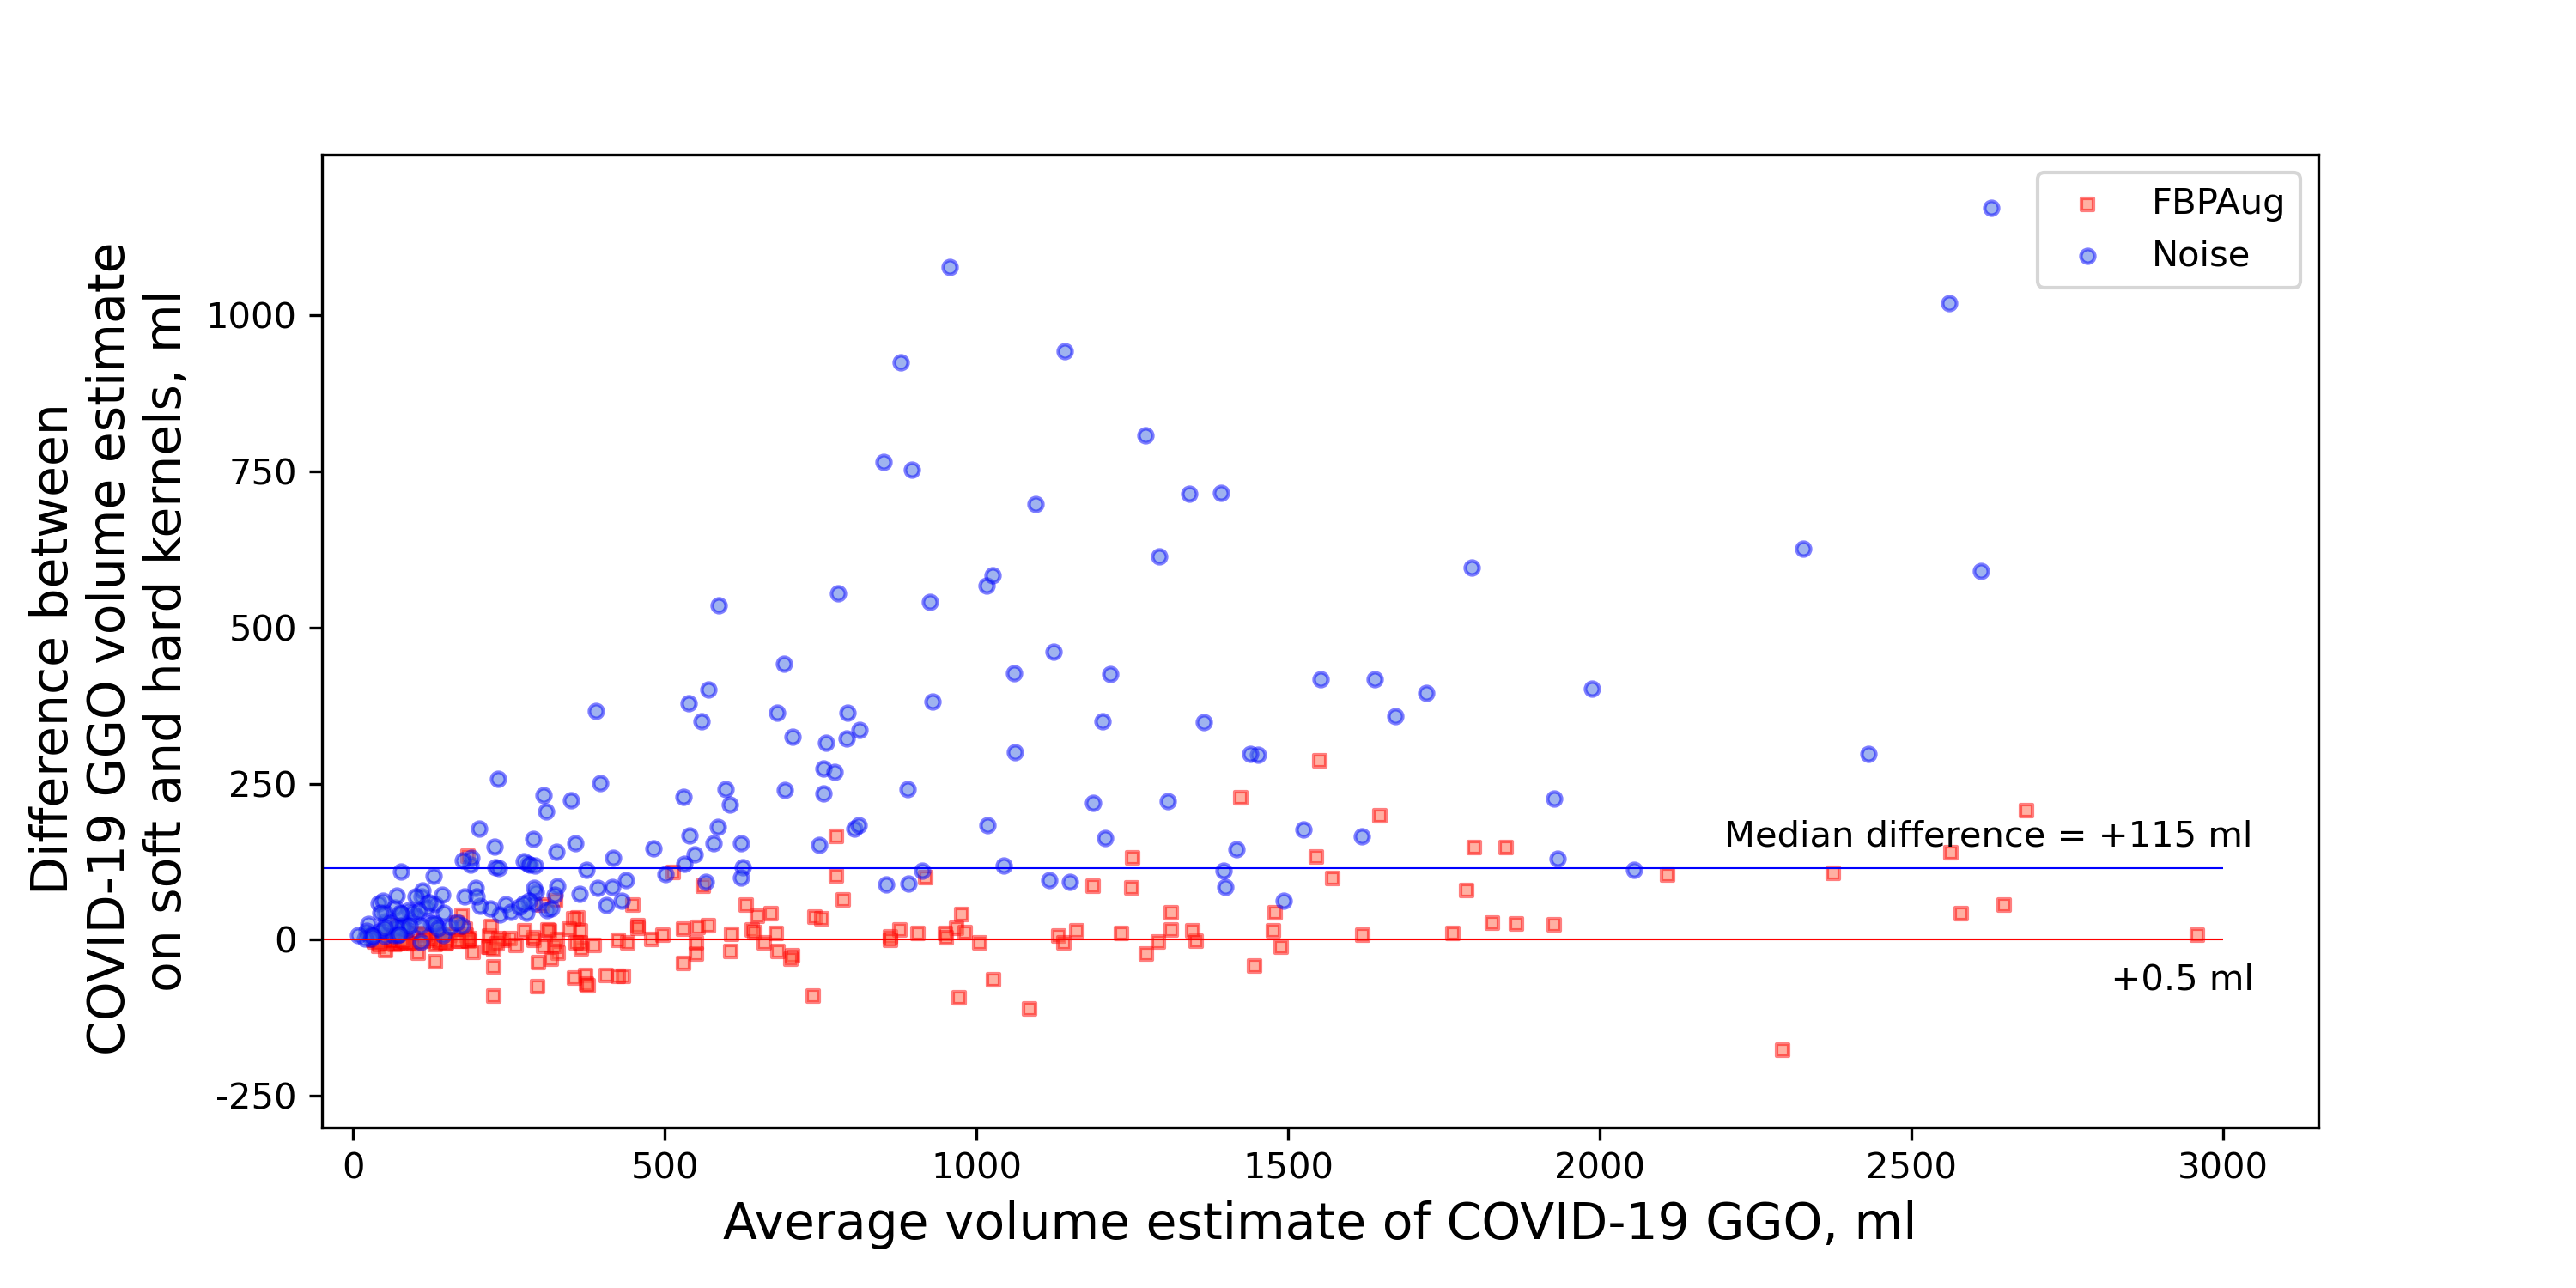
\includegraphics[width=\textwidth]{Dissertation/Figures/3_ct/bland-altman.png}
	\caption{Bland-Altman plot showing prediction agreement using FBPAug (proposed augmentation, red) and next best competitor (Gaussian noise, blue).}
	\label{fig:bland-altman}
\end{figure}

\begin{figure}[h]
	\centering
	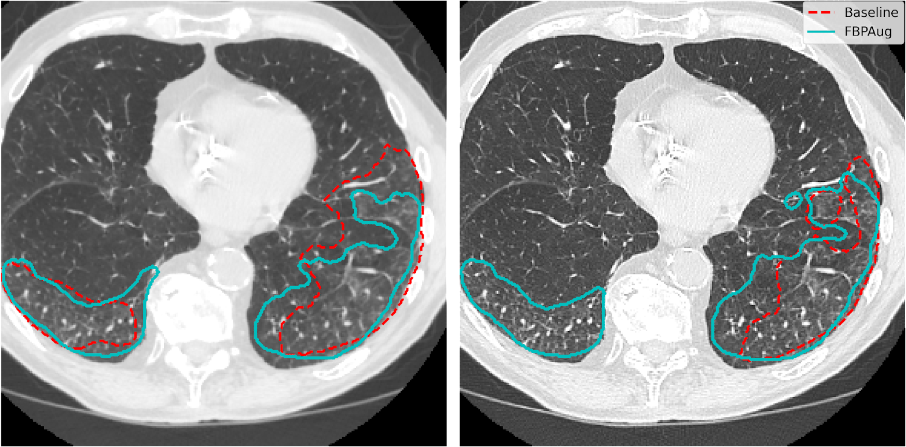
\includegraphics[width=\textwidth]{Dissertation/Figures/3_ct/contours_new.png}
	\caption{Example FBPAug predictions. Left -- image reconstructed with a \textit{smooth} kernel. Right -- image reconstructed with a \textit{sharp} kernel from the same sinogram.}
	\label{fig:fbpaug_pred}
	\vspace{2\baselineskip}
\end{figure}

\FloatBarrier % forces LaTeX to place all pending floats before continuing


\subsection{F-consistency experiments and results}

We compare some of the key results statistically using a one-sided Wilcoxon signed-rank test. We report p-values in two testing setups: $p_1$ -- comparing five mean values after cross-validation, and $p_2$ -- comparing Dice Scores on every image.% as an independent sample.


\textbf{Methods comparison.} To begin with, we show the existence of the domain shift problem within the COVID-19 segmentation task. The Dice Score of the baseline model on the COVID-test dataset is lower than the cross-validation score on the COVID-train dataset, $0.56$ against $0.60$. Also, this score is significantly lower than $0.64$ achieved by our adaptation method $\left(p_1 < 0.05,\: p_2 < 10^{-4} \right)$. See Table~\ref{tab:res_final}, comparing row Baseline to the others. For all adaptation methods, we observe an increase in the consistency score and segmentation quality on the target domain. Moreover, all methods maintain their quality on the source domain compared to Baseline.



%\begin{table}[H]
%	\caption{Comparison of all considered methods. The adaptation methods are trained using all training kernel pairs of the Paired-private dataset. F-/P-Cons stand for F-/P-Consistency, where F-Consistency is our proposed method. All results are Dice Scores in the format \textit{mean} $\pm$ \textit{std} calculated from $5$-fold cross-validation. We highlight the best scores in every column in \textbf{bold}.}
%	\begin{adjustwidth}{-\extralength}{0cm}
%		\newcolumntype{C}{>{\centering\arraybackslash}X}
%		\begin{tabularx}{\fulllength}{lCCCCCCC}
%			\toprule
%			
%			& \multirow{2.5}{*}{\textbf{COVID-train}} & \multirow{2.5}{*}{\textbf{COVID-test}} & \multicolumn{5}{c}{\textbf{Paired-Private} \textbf{Consistency}} \\
%			\cmidrule(lr){4-8}
%			& & & \textbf{FC07/55} & \textbf{FC07/51} & \textbf{SOFT/LUNG} & \textbf{STAND/LUNG}  & \textbf{Mean} \\
%			
%			
%			\midrule
%			Baseline & $\mathbf{0.60 \pm 0.04}$ & $0.56 \pm 0.03$ & $0.52 \pm 0.06$ & $0.39 \pm 0.07$ & $0.58 \pm 0.08$ & $0.28 \pm 0.05$ & $0.46 \pm 0.05$\\
%			
%			\cmidrule{1-8}
%			
%			FBPAug & $0.59 \pm 0.04$ & $0.62 \pm 0.03$ & $0.80 \pm 0.02$ & $0.71 \pm 0.03$ & $0.85 \pm 0.01$ & $0.65 \pm 0.03$ & $0.76 \pm 0.02$ \\
%			
%			
%			\cmidrule{1-8}
%			
%			%DANN (Dec) & $.57 \pm 0.04$ & $.61 \pm 0.04$ &  $.61 \pm 0.02$ & $.49 \pm 0.04$ & $.58 \pm 0.03$ & $.31 \pm 0.05$ & $.52 \pm 0.01$ \\
%			
%			%\cmidrule{1-8}
%			
%			DANN  & $0.58 \pm 0.05$ & $\mathbf{0.64 \pm 0.02}$ & $0.84 \pm 0.02$ & $0.70 \pm 0.02$ & $\mathbf{0.86 \pm 0.03}$ & $0.66 \pm 0.06$ & $0.78 \pm 0.02$ \\
%			
%			\cmidrule{1-8}
%			
%			P-Cons & $0.59 \pm 0.04$ & $0.61 \pm 0.01$ & $0.65 \pm 0.05$ & $0.60 \pm 0.02$ & $0.77 \pm 0.01$ & $0.47 \pm 0.04$ & $0.63 \pm 0.03$\\
%			
%			\cmidrule{1-8}
%			
%			
%			%F-Cons (Dec) & $\mathbf{.60 \pm 0.03}$ & $.58 \pm 0.02$ & $.62 \pm 0.05$ & $.54 \pm 0.03$ & $.75 \pm 0.01$ & $.40 \pm 0.06$ & $.58 \pm 0.02$ \\
%			
%			%\cmidrule{1-8}
%			
%			F-Cons &  $0.57 \pm 0.03$ & $\mathbf{0.64 \pm 0.03}$ & $\mathbf{0.88 \pm 0.01}$ & $\mathbf{0.72 \pm 0.04}$ & $0.83 \pm 0.02$ & $\mathbf{0.70 \pm 0.05}$ & $\mathbf{0.80 \pm 0.01}$ \\
%			
%			\bottomrule
%		\end{tabularx}
%		\label{tab:res_final}
%	\end{adjustwidth}
%\end{table}


\begin{table}[h]
	\centering
	\caption{Comparison of all considered methods, trained using all kernel pairs of the Paired-private dataset. All results are Dice Scores in the format \textit{mean (std)}.}
	\label{tab:res_final}
	%\resizebox{\textwidth}{!}{%
		\begin{tabular}{lcccccc}
			\toprule
			& \multirow{2.5}{*}{\shortstack{COVID-\\test}} & \multicolumn{5}{c}{Paired-private consistency} \\
			\cmidrule(lr){3-7}
			& & FC07/55 & FC07/51 & soft/lung & stnd/lung & mean \\
			\midrule
			
			Baseline & 0.56(0.03) & 0.52(0.06) & 0.39(0.07) & 0.58(0.08) & 0.28(0.05) & 0.46(0.05) \\
			
			\cmidrule{1-7}
			
			P-Cons & 0.61(0.01) & 0.65(0.05) & 0.60(0.02) & 0.77(0.01) & 0.47(0.04) & 0.63(0.03) \\
			
			\cmidrule{1-7}
			
			FBPAug & 0.62(0.03) & 0.80(0.02) & 0.71(0.03) & 0.85(0.01) & 0.65(0.03) & 0.76(0.02) \\
			
			\cmidrule{1-7}
			
			DANN & \textbf{0.64(0.02)} & 0.84(0.02) & 0.70(0.02) & \textbf{0.86(0.03)} & 0.66(0.06) & 0.78(0.02) \\		
			
			\cmidrule{1-7}
			
			F-Cons & \textbf{0.64(0.03)} & \textbf{0.88(0.01)} & \textbf{0.72(0.04)} & 0.83(0.02) & \textbf{0.70(0.05)} & \textbf{0.80(0.01)} \\
			
			\bottomrule
		\end{tabular}%}
\end{table}


% Further, we compare FBPAug to the best adaptation methods since it is a straightforward solution to the domain shift problem caused by the difference in the reconstruction kernels. Although FBPAug achieves comparable results on the target domain, F-Consistency outperforms it in terms of the average consistency score, $0.80$ Dice Score against $0.76$ $\left(p_1 < 0.05,\: p_2 < 10^{-5}\right)$. The results are also in Table~\ref{tab:res_final}, row FBPAug.

We compare P-Consistency (operating with the last layer) with F-Consistency and show that it results in the significantly lower consistency score, $0.63$ against $0.80$ $\left(p_1 < 0.05,\: p_2 < 10^{-10}\right)$. Thus, our findings align with the message of~\cite{zakazov2021anatomy} that the encoder layers contain more domain-specific information than the decoder ones.

F-consistency outperforms DANN. Although both methods score similar in target Dice Score, F-Consistency has an advantage over DANN in the consistency score: $0.80$ against $0.78$ $\left(p_1 < 0.05,\: p_2 < 10^{-2}\right)$. Our intuition here is F-Consistency explicitly enforces features alignment, while DANN enforces features to be indistinguishable for the discriminator. And the direct alignment appears to be more efficient.

We conclude comparison of the methods with the qualitative analysis. In Figure~\ref{fig:test_preds}, we provide examples of the Baseline, FBPAug, DANN, and F-Consistency predictions on the COVID-test dataset and compare them with the ground truth. All adaptation methods perform similar to the ground truth with minor inaccuracies, while Baseline gives massive false positive predictions on the unseen domain.%With the quantitative analysis above, these observations highlight the relevance of the domain adaptation problem in the COVID-19 segmentation task.

\begin{figure}[h]
	\centering
	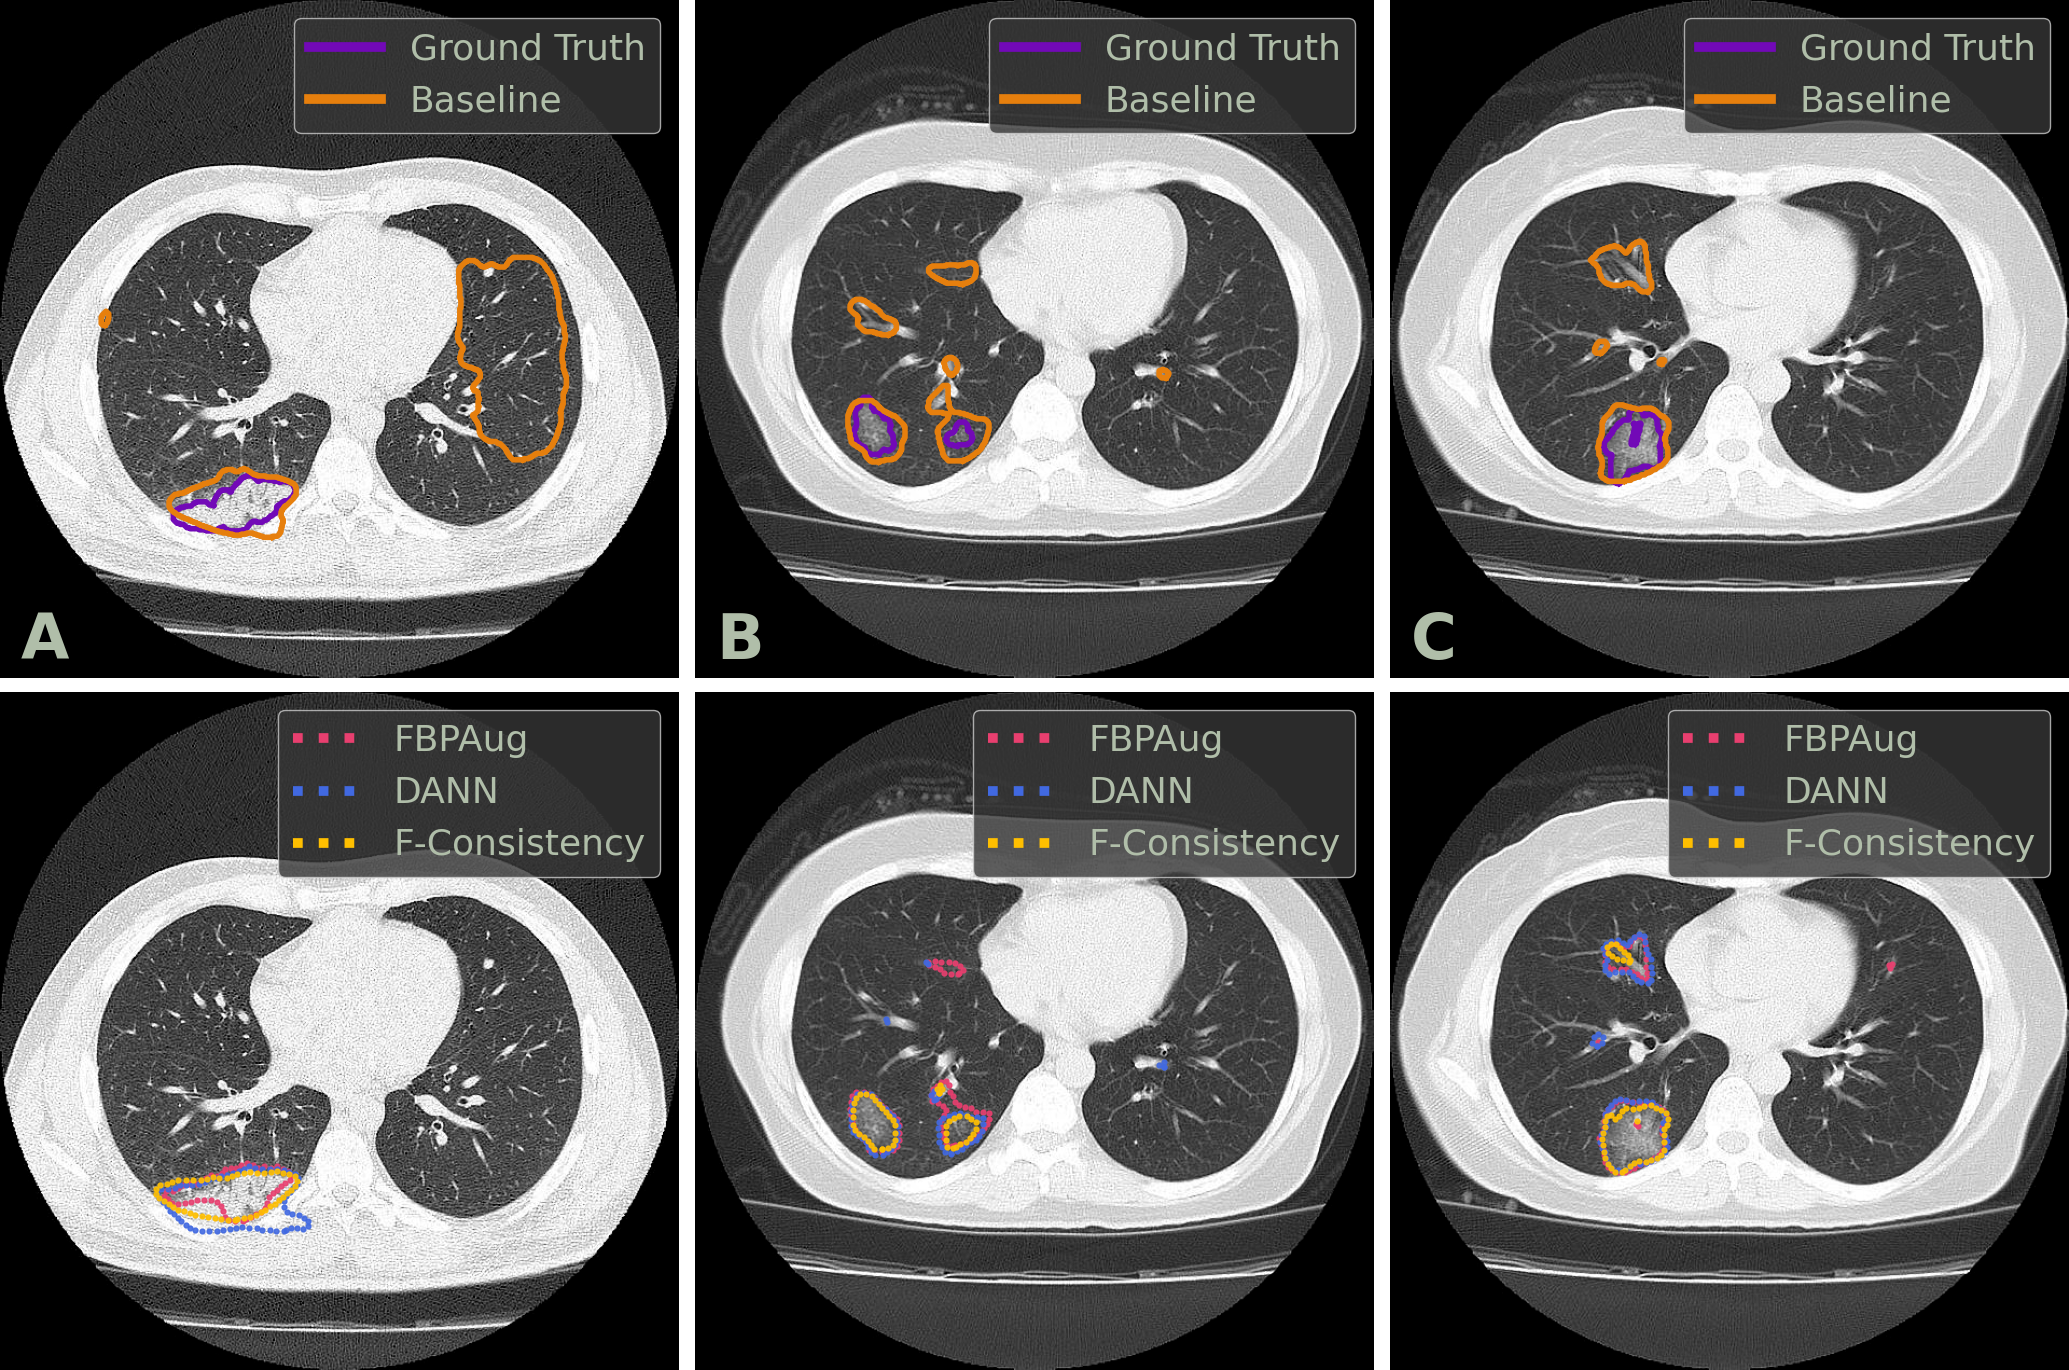
\includegraphics[width=\textwidth]{Dissertation/Figures/3_ct/test_preds.png}
	\caption{Examples of three axial CT slices (columns A, B, and C) from the COVID-test dataset with the corresponding predictions and ground truth annotations.}% Three columns, denoted \textbf{A}, \textbf{B}, and \textbf{C}, contains three unique slices.}% The top row contains the contours of the ground truth and baseline prediction. The bottom row contains the contours of the adaptation methods' predictions. DANN and F-Consistency correspond to DANN and F-Cons from Table~\ref{tab:res_final}, respectively.}
	\label{fig:test_preds}
\end{figure}

In Figure~\ref{fig:consistency_preds}, we visualize predictions on the paired images from the Paired-private dataset. For the Baseline, we observe an extreme inconsistency (Figure~\ref{fig:consistency_preds}~A) and massive false positive predictions in healthy lung tissues (Figure~\ref{fig:consistency_preds}~D) and outside lungs (Figure~\ref{fig:consistency_preds}~B). Predictions of the adaptation methods are visually more consistent inside every pair. Despite the high consistency scores, FBPAug and DANN output more aggressive predictions. FBPAug predicts motion artifacts near the body regions (Figure~\ref{fig:consistency_preds}~A) and triggers on healthy lung tissues (Figure~\ref{fig:consistency_preds}~B). DANN is more conservative but triggers on the consolidation-like tissues (Figure~\ref{fig:consistency_preds}~C,~D).% However, without the ground truth annotations on the paired data, we refer to this analysis as a discussion.

\begin{landscape}
\begin{figure}[p]
	% \centering
	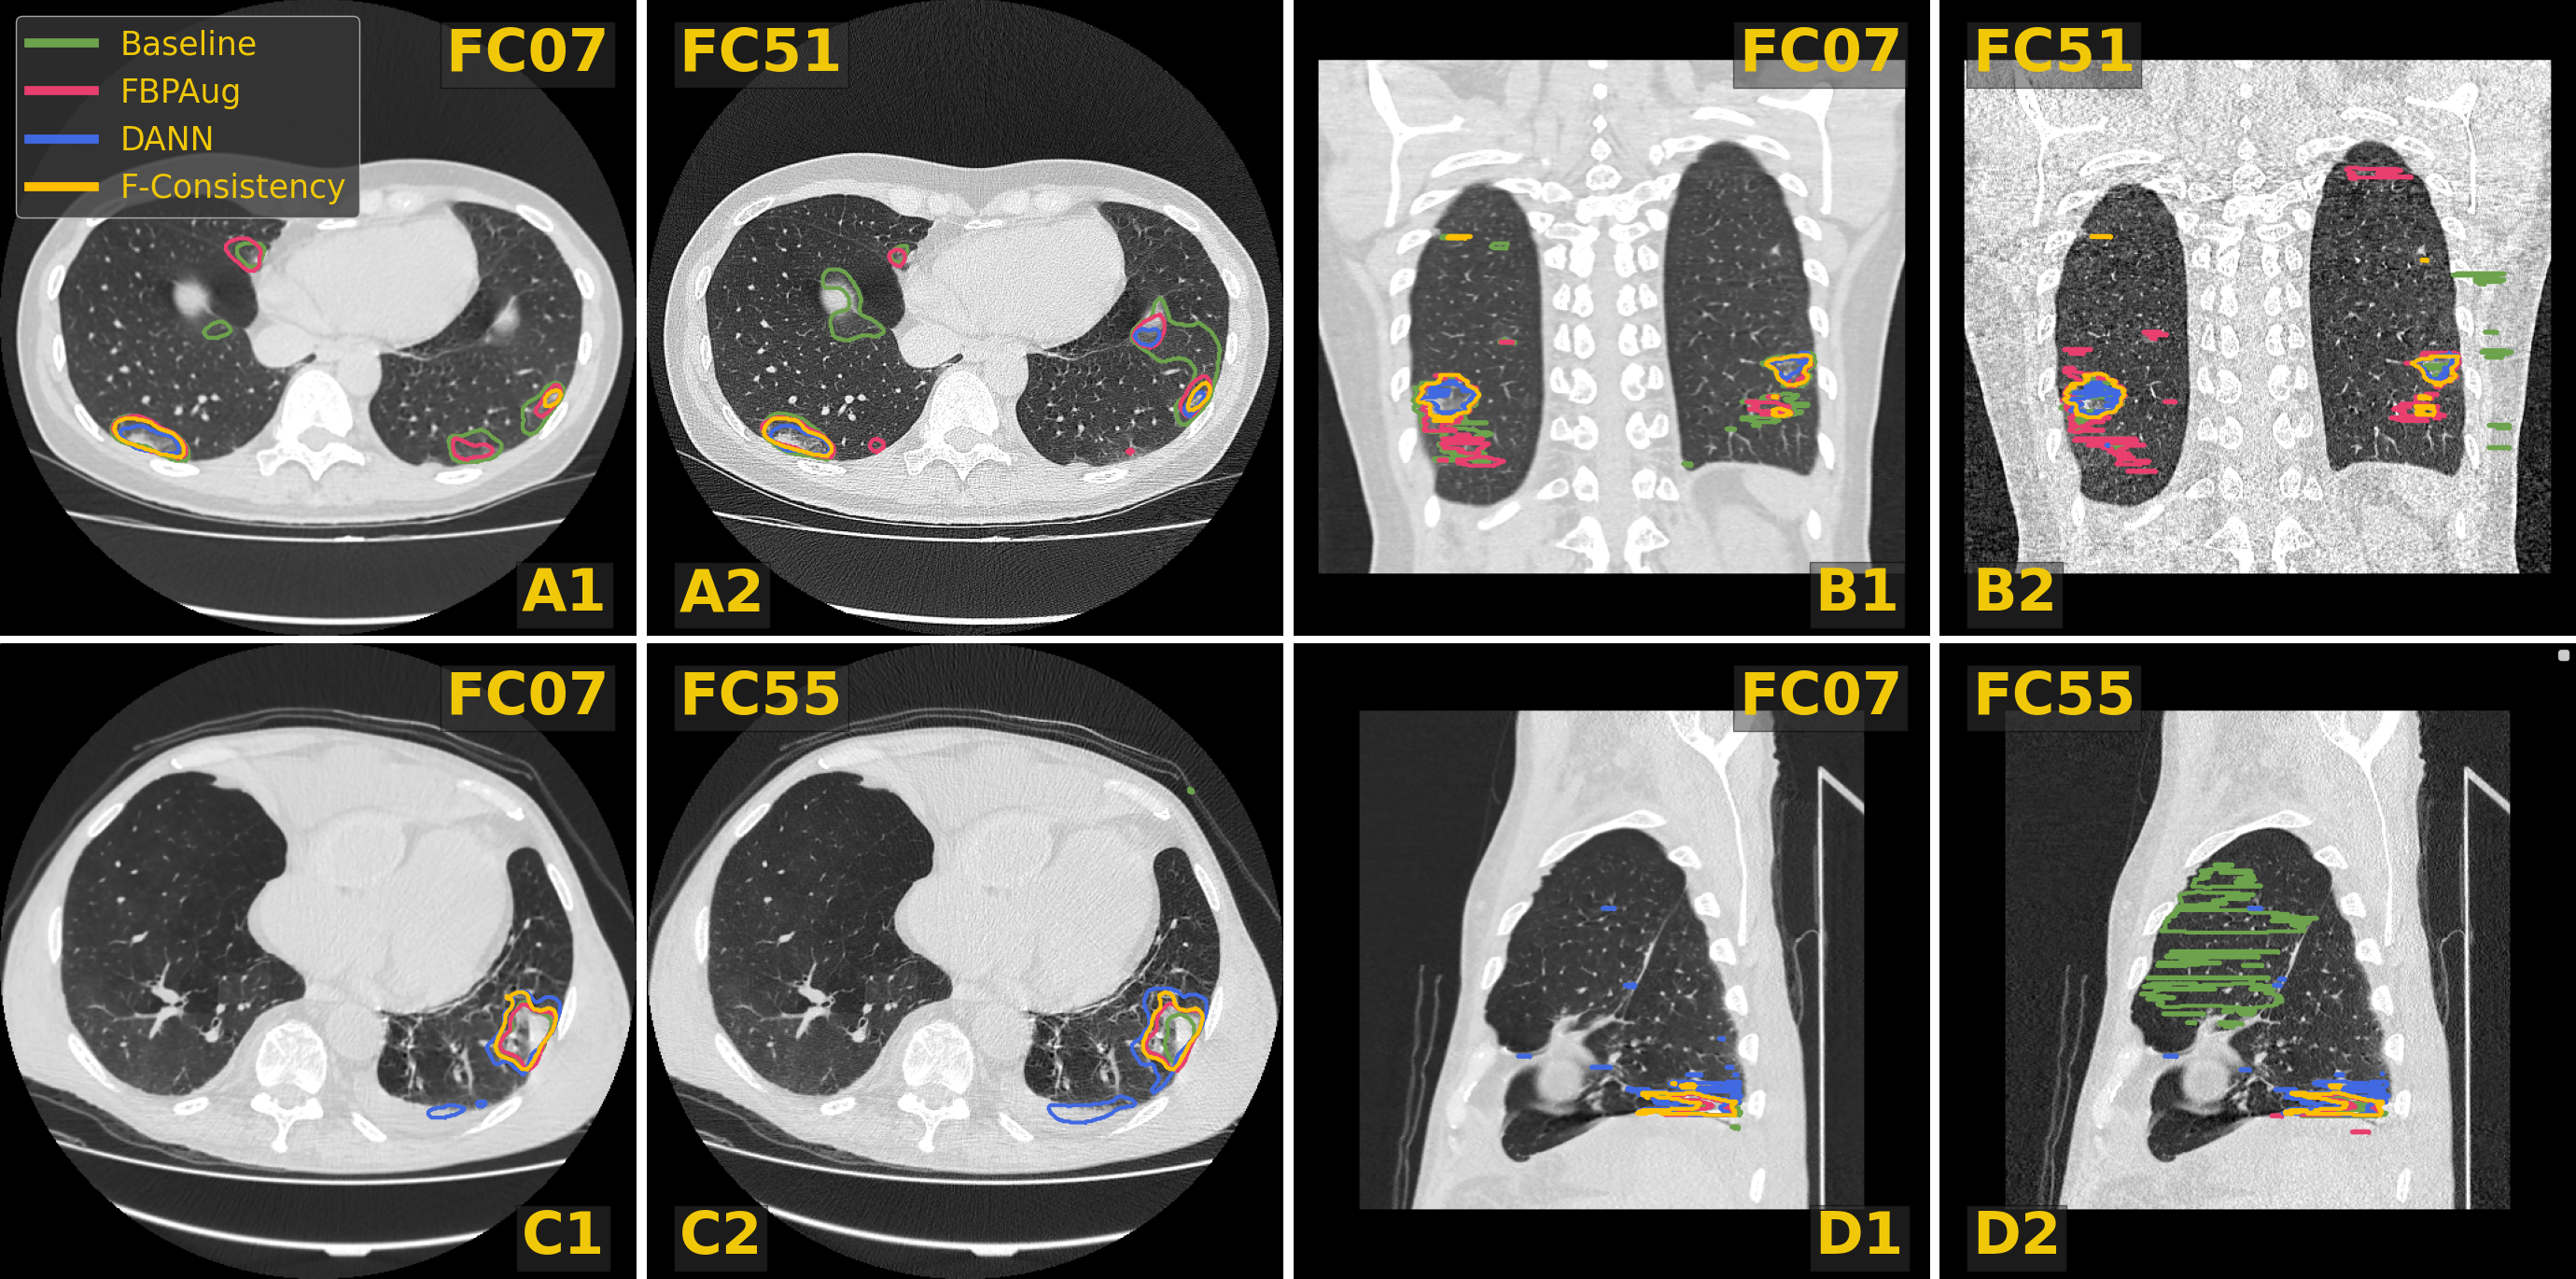
\includegraphics[width=\linewidth]{Dissertation/Figures/3_ct/consistency_preds.png}
	\caption{Examples of CT slices from the Private-paired dataset with the corresponding predictions on the paired images. Four doublets, denoted \textbf{A}, \textbf{B}, \textbf{C}, and \textbf{D}, contain corresponding slices from the smooth and sharp images. The doublets B and D are coronal and sagittal slices, respectively.}
	\label{fig:consistency_preds}
\end{figure}
\end{landscape}

%Below, we investigate the generalization of the models trained with fewer data and the trade-off between consistency and segmentation quality.


\textbf{Generalization with the less paired data.} We evaluate the models regularized using paired images from the Paired-public dataset. The dataset contains only FC07/FC51 and FC07/FC55 kernel pairs. Besides the previous setup, this data does not contain COVID-19 lesions. Thus, we show that some methods depend on the semantic content and poorly generalize to kernel styles. The results are shown in Table~\ref{tab:res_public}.



%\begin{table}[H]
%	\caption{Comparison of all adaptation methods from Table \ref{tab:res_final} except FBPAug trained on the Public-paired dataset. All results are Dice Scores in the format \textit{mean} $\pm$ \textit{std} calculated from $5$-fold cross-validation. We highlight the consistency scores near or below Baseline level in \textit{italic}. The best consistency scores are highlighted in \textbf{bold}.}
%	%\vspace{.2cm}
%	\begin{adjustwidth}{-\extralength}{0cm}
%		\newcolumntype{C}{>{\centering\arraybackslash}X}
%		\begin{tabularx}{\fulllength}{lCCCCCCC}
%			\toprule
%			
%			& \multirow{2.5}{*}{\shortstack{\textbf{COVID-Train}}} & \multirow{2.5}{*}{\textbf{COVID-Test}}& \multicolumn{5}{c}{\textbf{Paired-Private} \textbf{Consistency}} \\
%			\cmidrule(lr){4-8}
%			&  & & \textbf{FC07/55} & \textbf{FC07/51} & \textbf{LUNG/SOFT }& \textbf{LUNG/STAND }  & \textbf{Mean}\\
%			
%			\midrule
%			Baseline & $\mathbf{0.60 \pm 0.04}$ & $0.56 \pm 0.03$ & $0.52 \pm 0.06$ & $0.39 \pm 0.07$ & $0.58 \pm 0.08$ & $0.28 \pm 0.05$ & $0.46 \pm 0.05$\\
%			
%			% \cmidrule{1-8}
%			
%			% DANN (Dec) & $0.58 \pm 0.04$ & $0.63 \pm 0.04$ & $.62 \pm 0.03$ & $.49 \pm 0.07$ & $\mathit{.60 \pm 0.03}$ & $\mathit{.30 \pm 0.04}$ & $\mathit{.53 \pm 0.03}$ \\
%			
%			\cmidrule{1-8}
%			
%			% DANN & $.58 \pm 0.05$ & $.64 \pm 0.02$ & $.84 \pm 0.02$ & $.70 \pm 0.02$ & $.86 \pm 0.03$ & $.66 \pm 0.06$ & $.78 \pm 0.02$ \\
%			
%			% \cmidrule{1-8}
%			
%			DANN &  $\mathbf{0.60 \pm 0.03}$ &  $\mathbf{0.64 \pm 0.02}$ & $0.75 \pm 0.02$ & $\mathbf{0.64 \pm 0.05}$ & $0.67 \pm 0.03$ & $0.50 \pm 0.05$  & $0.66 \pm 0.02$ \\
%			
%			\cmidrule{1-8}
%			
%			% P-Cons & $0.59 \pm 0.04$ & $0.61 \pm 0.01$ & $0.65 \pm 0.05$ & $0.60 \pm 0.02$ & $0.77 \pm 0.01$ & $0.47 \pm 0.04$ & $0.63 \pm 0.03$\\
%			
%			% \cmidrule{1-8}
%			
%			P-Cons & $0.53 \pm 0.03$ & $0.58 \pm 0.03$ & $\mathit{0.54 \pm 0.05}$ & $\mathit{0.44 \pm 0.03}$ & $\mathit{0.57 \pm 0.04}$  & $\mathit{0.28 \pm 0.06}$ & $\mathit{0.47 \pm 0.03}$  \\
%			
%			\cmidrule{1-8}
%			
%			% F-Cons (Dec) & $0.60 \pm 0.03$ & $0.59 \pm 0.00$ & $\mathit{.54 \pm 0.05}$ & $\mathit{.47 \pm 0.05}$ & $\mathit{.64 \pm 0.05}$ & $\mathit{.31 \pm 0.06}$ &  $\mathit{.50 \pm 0.04}$ \\
%			
%			% \cmidrule{1-8}
%			
%			% F-Cons &  $0.57 \pm 0.03$ & $0.64 \pm 0.03$ & $0.88 \pm 0.01$ & $0.72 \pm 0.04$ & $0.83 \pm 0.02$ & $0.70 \pm 0.05$ & $0.80 \pm 0.01$ \\
%			
%			% \cmidrule{1-8}
%			
%			F-Cons & $0.59 \pm 0.04$ & $\mathbf{0.64 \pm 0.02}$ & $\mathbf{0.80 \pm 0.02}$ & $\mathbf{0.63 \pm 0.04}$ & $\mathbf{0.71 \pm 0.02}$ & $\mathbf{0.55 \pm 0.05}$ & $\mathbf{0.70 \pm 0.02}$  \\
%			
%			\bottomrule
%		\end{tabularx}
%		\label{tab:res_public}
%	\end{adjustwidth}
%\end{table}


\begin{table}[h]
	\centering
	\caption{Comparison of adaptation methods trained on the Public-paired dataset. All results are Dice scores in the format \textit{mean (std)} calculated from $5$-fold cross-validation.}
	%\vspace{.2cm}
	%\resizebox{\textwidth}{!}{%
		\begin{tabular}{lcccccc}
			\toprule
			& \multirow{2.5}{*}{\shortstack{COVID-\\test}} & \multicolumn{5}{c}{Paired-private consistency} \\
			\cmidrule(lr){3-7}
			& & FC07/55 & FC07/51 & soft/lung & stnd/lung & mean \\
			\midrule
			
			Baseline & 0.56(0.03) & 0.52(0.06) & 0.39(0.07) & 0.58(0.08) & 0.28(0.05) & 0.46(0.05) \\
			
			\cmidrule{1-7}
			
			P-Cons & 0.58(0.03) & 0.54(0.05) & 0.44(0.03) & 0.57(0.04) & 0.28(0.06) & 0.47(0.03) \\
			
			\cmidrule{1-7}
			
			DANN & \textbf{0.64(0.02)} & 0.75(0.02) & \textbf{0.64(0.05)} & 0.67(0.03) & 0.50(0.05) & 0.66(0.02) \\
			
			\cmidrule{1-7}
			
			F-Cons & \textbf{0.64(0.02)} & \textbf{0.80(0.02)} & 0.63(0.04) & \textbf{0.71(0.02)} & \textbf{0.55(0.05)} & \textbf{0.70(0.02)} \\
			
			\bottomrule
		\end{tabular}%}
		\label{tab:res_public}
\end{table}

We highlight two main findings from these results. Firstly, consistency of the method that operates with the decoder layers decreases to the level of Baseline; see P-Consistency in Table~\ref{tab:res_public}. Our intuition here is that the decoder version of the model can be more easily enforced to output the trivial predictions than the encoder one. Simultaneously, the images without COVID-19 lesions induce trivial predictions. Therefore, it might be easier for these models to differ the paired dataset from the source dataset by the semantic content and fail to align the stylistic features.

Finally, we observe our method, F-Consistency, to outperform the other adaptation methods training only on the publicly available data. At this point, FBPAug (Table~\ref{tab:res_final}) outperforms the adaptation methods. The latter indicates that the range of synthetically augmented data overlaps the range of Paired-public. So, if we have a large and representative set of paired data, enforcing consistency, as proposed F-consistency does, provides the best adaptation results. On the other hand, we can use the proposed augmentation method, FBPAug, in a zero-shot adaptation regime to achieve competitive performance if enough paired data is not provided.


\section{Summary}

We have proposed a new knowledge-driven augmentation method, FBPAug, to eliminate CT domain shifts related to the usage of different reconstruction kernels. It outperforms existing augmentation approaches and, in a zero-shot regime, other adaptation approaches. We also release the code, so FBPAug can be easily incorporated into any existing deep learning pipeline to ensure zero-shot domain adaptation in CT images.

Secondly, we have proposed an unsupervised domain adaptation method, F-Consistency, to address the same domain shift in CT reconstruction kernels. Our method uses a set of unlabeled CT image pairs and enforces the similarity between feature maps of paired images. We have shown that F-Consistency outperformed the other adaptation methods and FBPAug in the COVID-19 segmentation task \textit{when provided with enough unlabeled data}. Finally, through extensive evaluation, we have shown our method to generalize to the unseen reconstruction kernels better and without the specific semantic content.


